\section{Exercises 301}
\subsection{RDP Curve Simplification}
The Ramer-Douglas-Peucker (RDP) algorithm is a recursive curve simplification algorithm that works (naively) by preserving prominent curvature while accounting for the scale of the curve itself.  

 
\subsection{Point to Line Segment Distance}

One way to simplify a curve defined by points $v_1, . . ., v_n$ is by essentially considering curvature as deviation from a line segment.   Therefore, let us first consider the \textit{distance to the line segment} problem. Given a point $x \in R^2$, let's derive an expression for the distance between $x$ and its closest points on the line segment defined by endpoints $v_1, v_2 \in \R^2$:

 The vector $s$ from $v_1$ to $v_2$ can be described as $s= v_2 - v_1$ and the vector $u$ from $v_1$ to $x$ as $u = vx - v_1$.  We now project $u$ onto $s$ to give the closest point on the \emph{line}. 

Recall that one can represent any point on a \emph{line segment} parametrically by
\[p(t) = (1 -t)v_1 + tv_2 \quad \text{for} \quad   0 \leq t \leq 1.\]

Then our projection of $u$ onto $s$ gives a position $$ t = \frac{\mathbf{u} \cdot \mathbf{s}}{\mathbf{s} \cdot \mathbf{s}} = \frac{(\mathbf{x} - \mathbf{v}_1) \cdot (\mathbf{v}_2 - \mathbf{v}_1)}{(\mathbf{v}_2 - \mathbf{v}_1) \cdot (\mathbf{v}_2 - \mathbf{v}_1)}. $$ 
from $v_1$ along the direction of $s$ and our closest point on the line segment


$$\mathbf{p}_{closest} = \begin{cases} 
v_1  & \text{if }  t < 0\\
v_2  & \text{if } t > 1 \\
p(t) = v_1 + ts & \text{if } 0 \leq t \leq 1
 \end{cases} $$


where $t=\frac{(\mathbf{x}-\mathbf{v}_{1})\cdot (\mathbf{v}_{2}-\mathbf{v}_{1})}{(\mathbf{v}_{2}-\mathbf{v}_{1})\cdot (\mathbf{v}_{2}-\mathbf{v}_{1})}$.  We now apply the Euclidean distance formula 
$||x - p_{closest}||$
to determine the distance between $x$ and $p_{closest}$.  \\


More algorithmically, to solve the distance to line segment problem:
\begin{enumerate}
    \item Calculate the parameter $t$
    \item Determine the case for $p_{closest}$ based on the value of $t$
    \item Apply the Euclidean Distance Formula for $x$ and $p_{closest}$
\end{enumerate}

\begin{marginfigure}
   \centering
   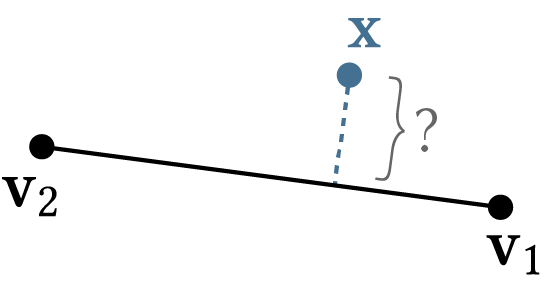
\includegraphics[width=0.8\linewidth]{images/SegmentDistance.png}
   \caption{In this picture, our $p_{closest}$ is the point $p(t) = v_1 + ts$, where $t=\frac{(\mathbf{x}-\mathbf{v}_{1})\cdot (\mathbf{v}_{2}-\mathbf{v}_{1})}{(\mathbf{v}_{2}-\mathbf{v}_{1})\cdot (\mathbf{v}_{2}-\mathbf{v}_{1})}$.}  
\end{marginfigure}

\subsection{Qaudratic Error Curve Simplification}

